\documentclass[11pt,a4paper,oneside]{article}
\usepackage[T1]{fontenc}
\usepackage[utf8]{inputenc}
\usepackage[french,english]{babel}
\usepackage[babel=true,kerning=true]{microtype}
\usepackage[usenames,dvipsnames,svgnames,table]{xcolor}
\usepackage[colorlinks,linkcolor={blue!30!black},citecolor={blue!50!black},urlcolor={blue!80!black}]{hyperref}
\usepackage{amsmath,amsfonts,amssymb,array,graphicx,caption,lmodern,subcaption,tikz,url,xspace,wrapfig}
\usepackage{textcomp,rotating,epic,pdfpages,listings,diagbox,multirow,float}

\usepackage[top=15mm,bottom=15mm,left=20mm,right=20mm]{geometry}

\parskip=6pt % adds vertical space between paragraphs

\DeclareMathOperator{\e}{e}

\begin{document}

\pagenumbering{gobble}  % Pas de numérotation
\begin{titlepage}
    \vspace*{50px}
    
\includegraphics[height=80px]{Images/logo_phelma.pdf}
    \vspace*{-80px}
\begin{flushright}
%     \vspace*{60px}
    
\includegraphics[height=65px]{Images/CIME.jpg}
\end{flushright}

\vspace*{2cm}

\begin{center}
\rule{\linewidth}{0.5mm}\\[0.4cm]
{\huge{\bfseries Compte Rendu}\\[0.4cm]
\textsc{TP Simulation électronique}\\[0.4cm]}
\rule{\linewidth}{0.5mm}\\[0.5cm]

\LARGE{\textsc{Nicolas Paillet, Félix Piédallu \& Giulia Rizzo}}\\[0.7cm]
\large{\textsc{2015-2016}}\\[2cm]

\Large{~}\\[1cm]
% 
\includegraphics[width=0.4\textwidth]{Images/CIME.jpg}\\[1cm]
%
 \large{Encadrant : Marco Pala}\\[2cm]
%

\end{center}
\end{titlepage}

\tableofcontents        % Table des matières avec liens, générée automatiquement.
\newpage
\pagenumbering{arabic}  % Numérotation de retour !


\section*{Introduction}
\addcontentsline{toc}{section}{Introduction}

Extended X-ray Absorption Fine Structure (EXAFS) is a spectroscopic method to caracterize elements of a sample (fluid or solid). The sample is placed on the trajectory of a X-ray beam, insensity of the X-ray is mesured before and after the sample, it give us absorption of the X-ray produced by passing through the sample.\\
The sample is scanned by X-rays of differents energies. In the EXAFS domain, kinetic enregy of photoelectron sent is from 50 eV to 1000 eV approximatively.

This study is composed of two parts: Firstly, we are going to devellop theorical aspects of the EXAFS and working principle of the CERN used. Secondly, how to make standards samples and exploitations of results.




\newpage

\section{Theorical aspects}
\subsection{EXAFS Domain and utilisation}
\subsubsection{Atomic X-Ray absorption}
When interacting with matter, X-Rays are absorbed by atoms, resulting into an electron excitation.

If the incident X-Ray beam has a greater energy than the binding energy of a core-level electron, this electron is ejected from the atom into the continuum, leaving the atom with a core hole.\\This is the Photoelectric effect.

The atom will relax from this excited state through two main processes : X-Ray Fluorescence and Auger Effect.

\paragraph{The Auger Effect :} To fill the core hole, an electron drops into it. The dissipated energy is asborbed by a second electron, thus ejected from a higher energy core-level into the continuum.

\paragraph{The X-Ray Fluorescence :} As in the Auger Effect, an electron drops into the core hole from a higher energy core-level, while emmiting an X-Ray beam of the energy gap between the core levels.

Those two effects result into a quasi-linear absorption coefficient :
\[\mu \simeq \frac{\rho Z^4}{A E^3}\]
\begin{figure}[h]
    \begin{center}
        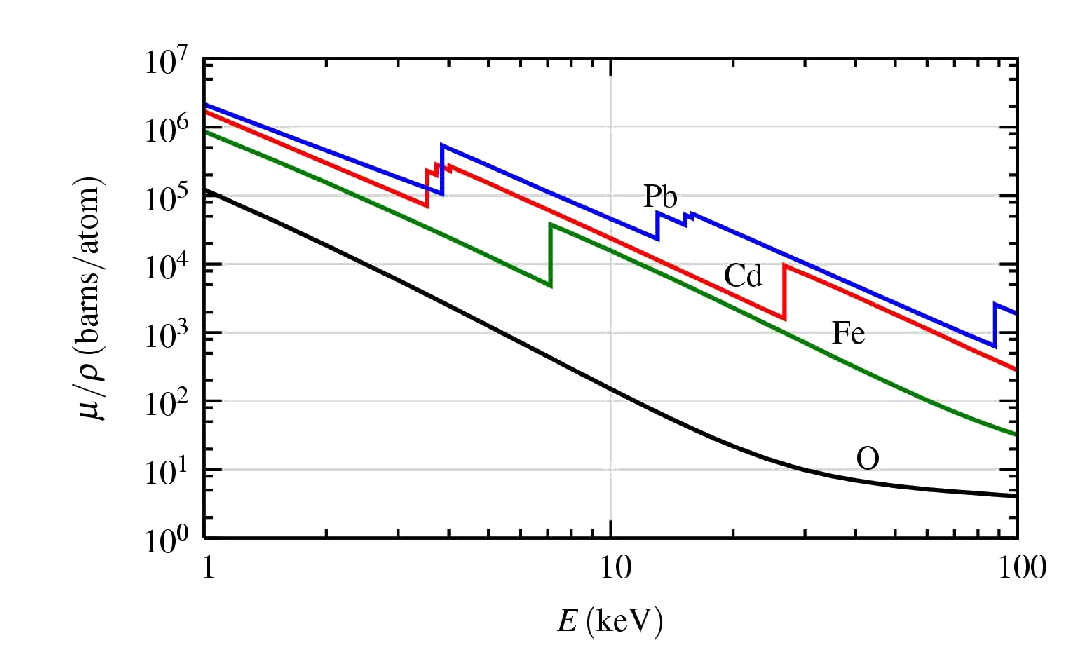
\includegraphics[width=0.7\textwidth]{Images/AbsorptionCoeff}
        \caption{The X-Ray absorption coefficient for Pb, Cd, Fe and O.}
        \label{absorptionCoeff}
    \end{center}
\end{figure}

The "edges" in this graph result from the electronic energy levels of the element : for each edge, another core level can absorb the X-Ray, as the incident energy becames enough to excitate the level.

\newpage
\subsubsection{The XAFS phenomenon}
For an isolated atom, the absorption edges are perfectly sharp, and $\mu(E)$ is smooth above the edges.

But in condensed matter, the absorbing atom is surrounded by other atoms (same or different) : the emitted photoelectron can scatter from neighbouring atoms and come back to the first atom.

The outgoing and ingoing waves of the back-scattered photoelectron will interfere, thus modulating the absorption coefficient of the atom (Fig. \ref{scatteringschema}).
\begin{figure}[h]
    \begin{center}
        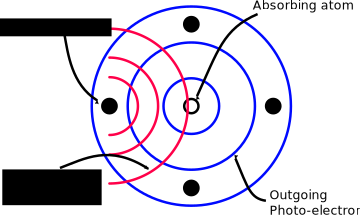
\includegraphics[width=0.5\textwidth]{Images/Scattering}
        \caption{A photo-electron emitted (blue) and back-scattered (red) to the central atom}
        \label{scatteringschema}
    \end{center}
\end{figure}

This modulation is easily visible on the Figure \ref{exafsgraph}. We will define the normalised EXAFS oscillations :
\[\chi(E) = \frac{\mu(E) - \mu_0(E)}{\Delta\mu_0(E_0)}\]
with $\mu_0(E)$ the "smooth background" of the isolated atom, and $\Delta\mu_0(E_0)$ the edge step or "jump".

\begin{figure}[h]
    \begin{center}
        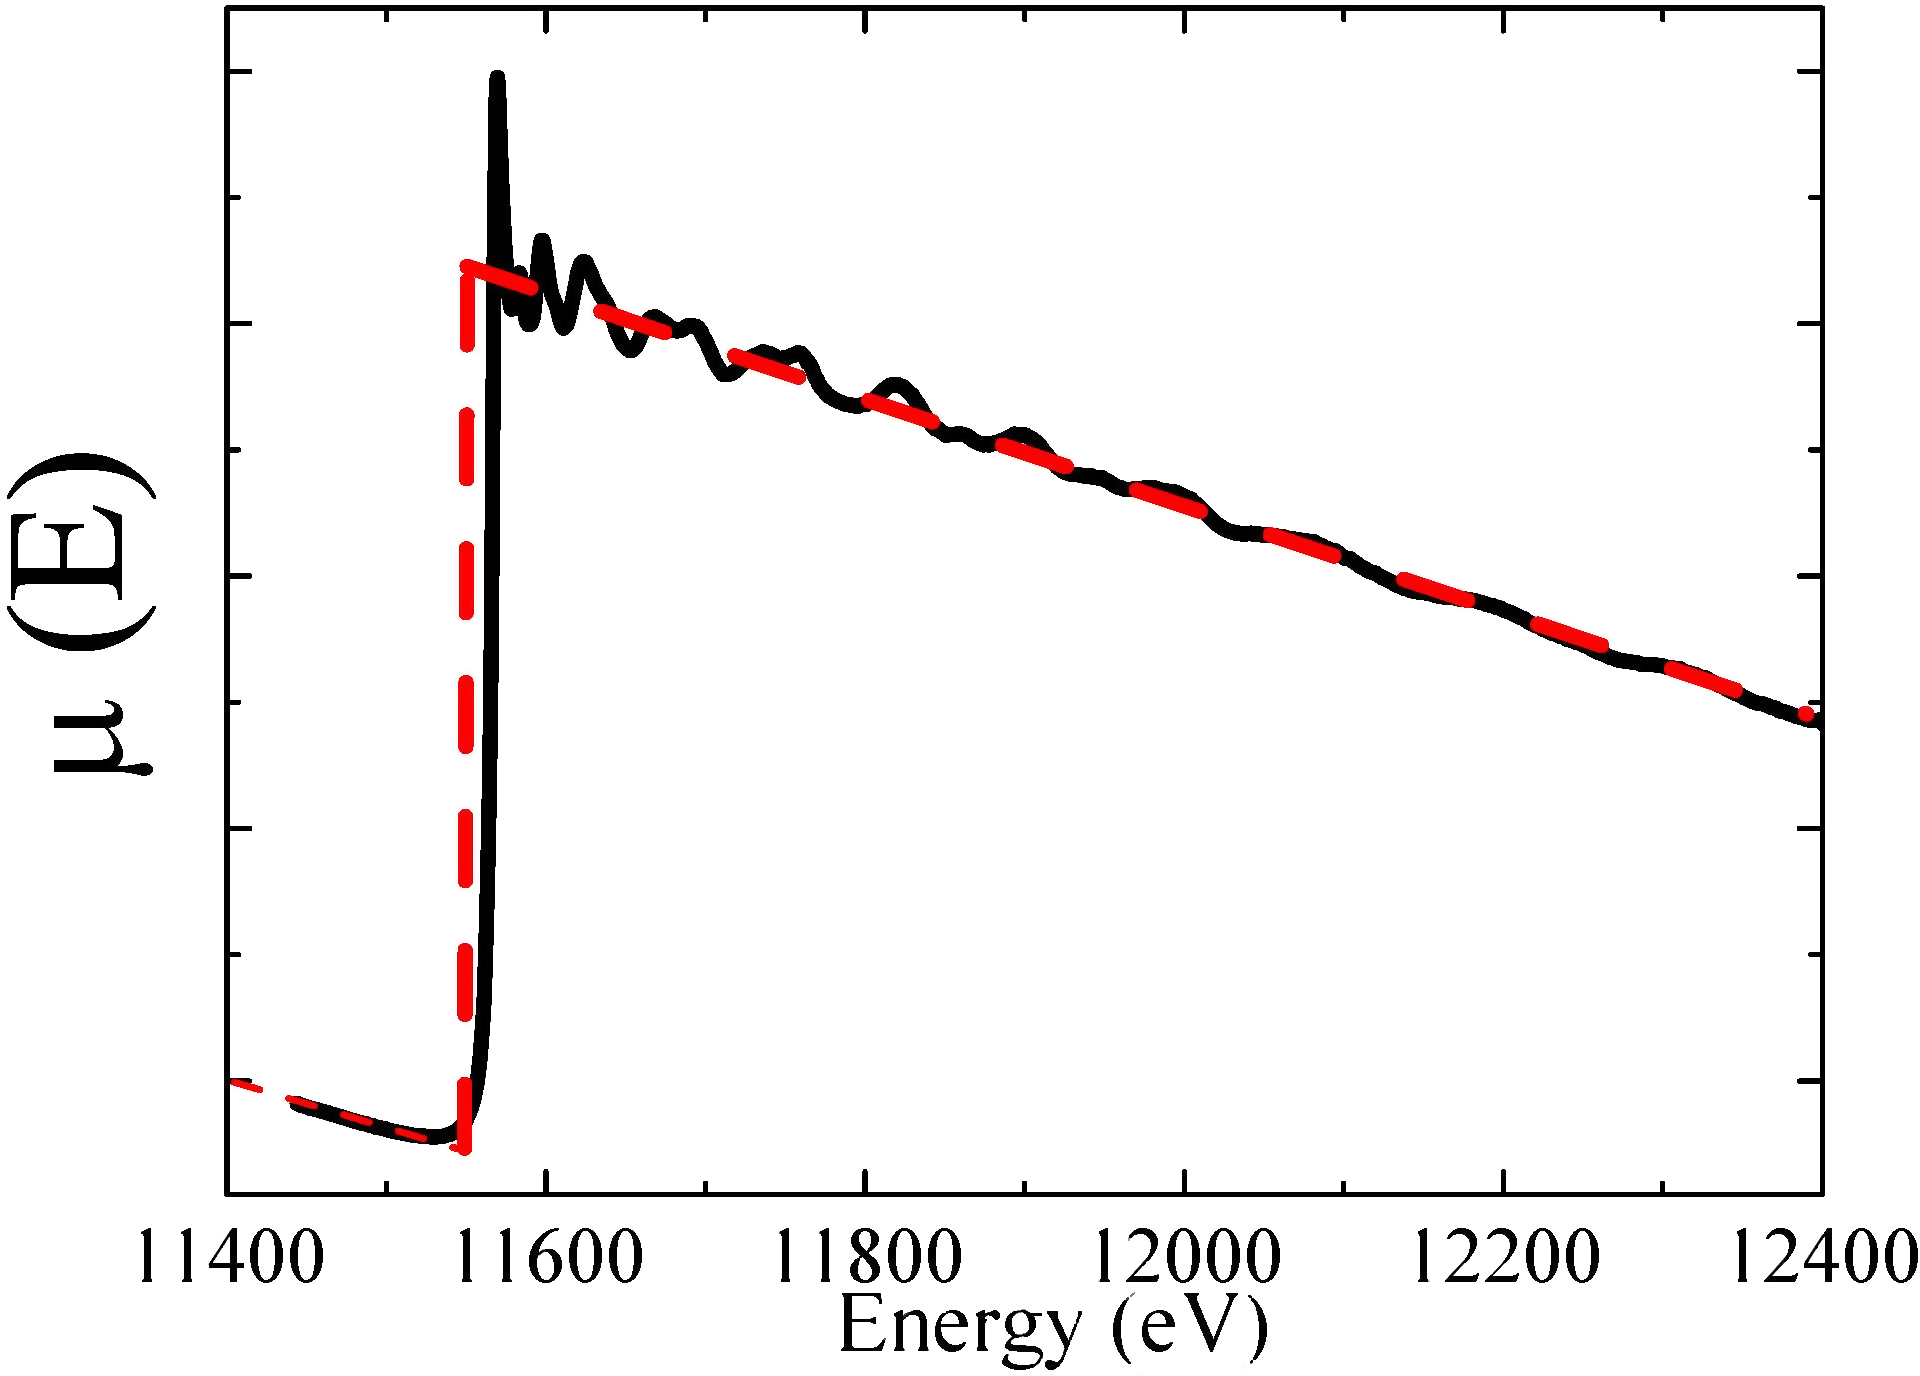
\includegraphics[height=0.35\textwidth]{Images/EXAFS2}
        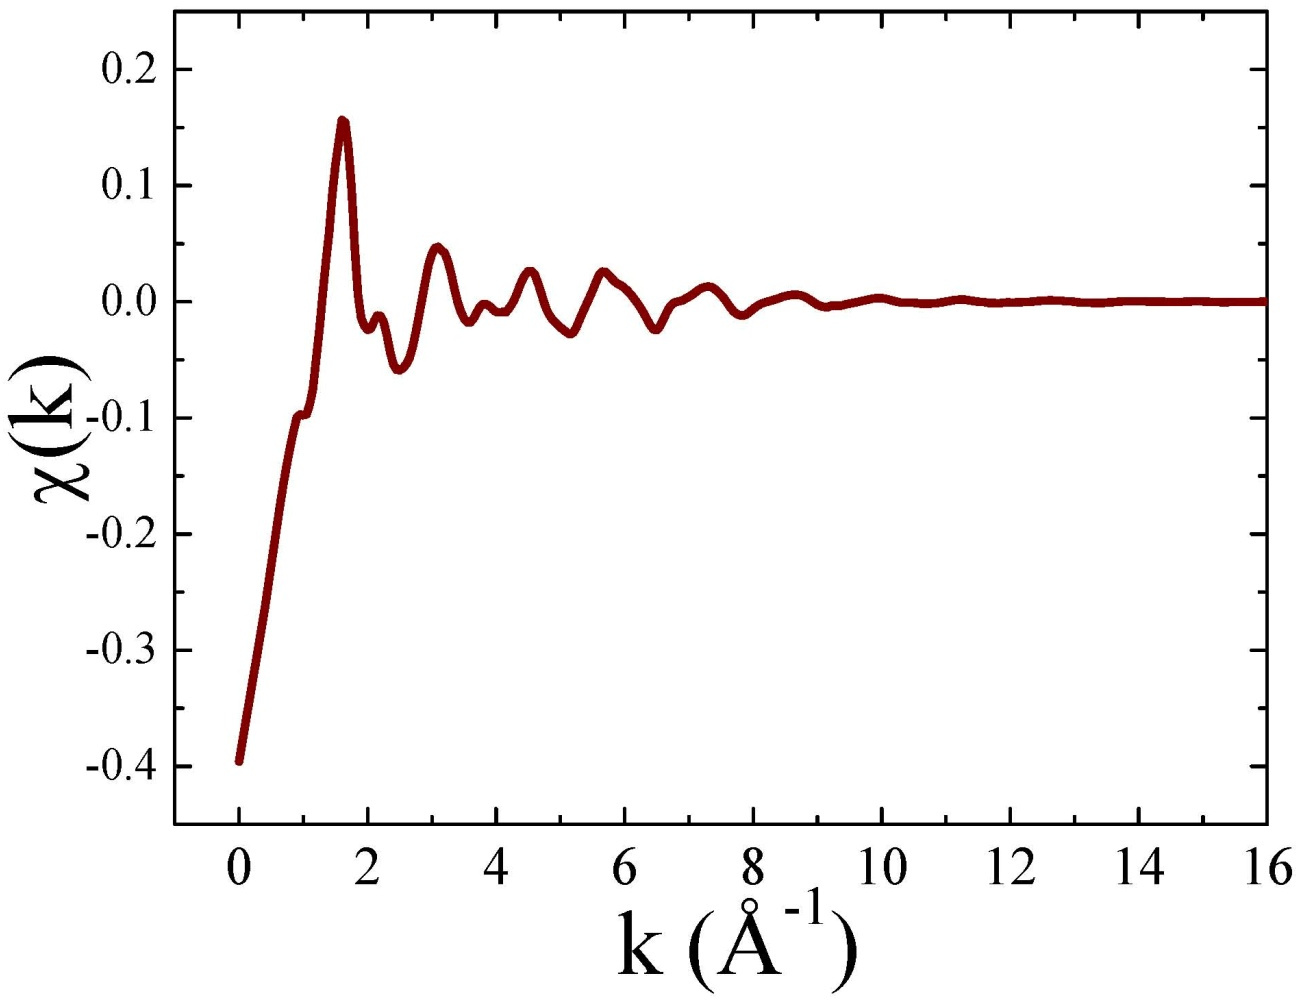
\includegraphics[height=0.35\textwidth]{Images/relativeEXAFS}
        \caption{EXAFS phenomenon, raw and normalised}
        \label{exafsgraph}
    \end{center}
\end{figure}


\newpage
\subsection{Grenoble CERN Operating principle}

The ESRF is a synchrotron, so it is mostly coposed by a LINear ACcelerator (LINAC), a booster ring and a storage ring.
\begin{itemize}
    \item LINAC: At the beginning, an electron gun make electron and send them to the LINAC where their are accelerate by an alectromagnetic fiels that attract them. At the ESRF, electron gun is a 100 keV triode gun and there are two 6 meter acceleration sections of 35 MW each to put electrons at 200 MeV.
    \item Booster ring: when electron have made their pre-acceleration in the LINAC, their enter in the booster ring (300 meter circumference) to be accelerated near to light speed at 6 GeV.
    \item Storage ring: It is the last and biggest ring (844.4 meter circumference). In this ring, electron alternate straight lines and bending sections. The ESRF synchrotron strorage ring is composed by 64 bending magnets and on straight lines, there are 320 quadrupoles to keep the beam focused, 224 sextupoles to avoid chromatic aberration, undulators and wigglers both force electrons to have a sinusoidal trajectory instead of straight one.
\end{itemize}
\medskip

Like we have seen in the part \ref{theory}, when electrons turn, there emit X-rays breaking radiation. That X-rays are capted to make experiments on beamlines.\medskip


The Hall where all experiments lines (beamlines) are regrouped is in the figure \ref{Hall}.\medskip

\begin{figure}[H]
    \begin{center}
        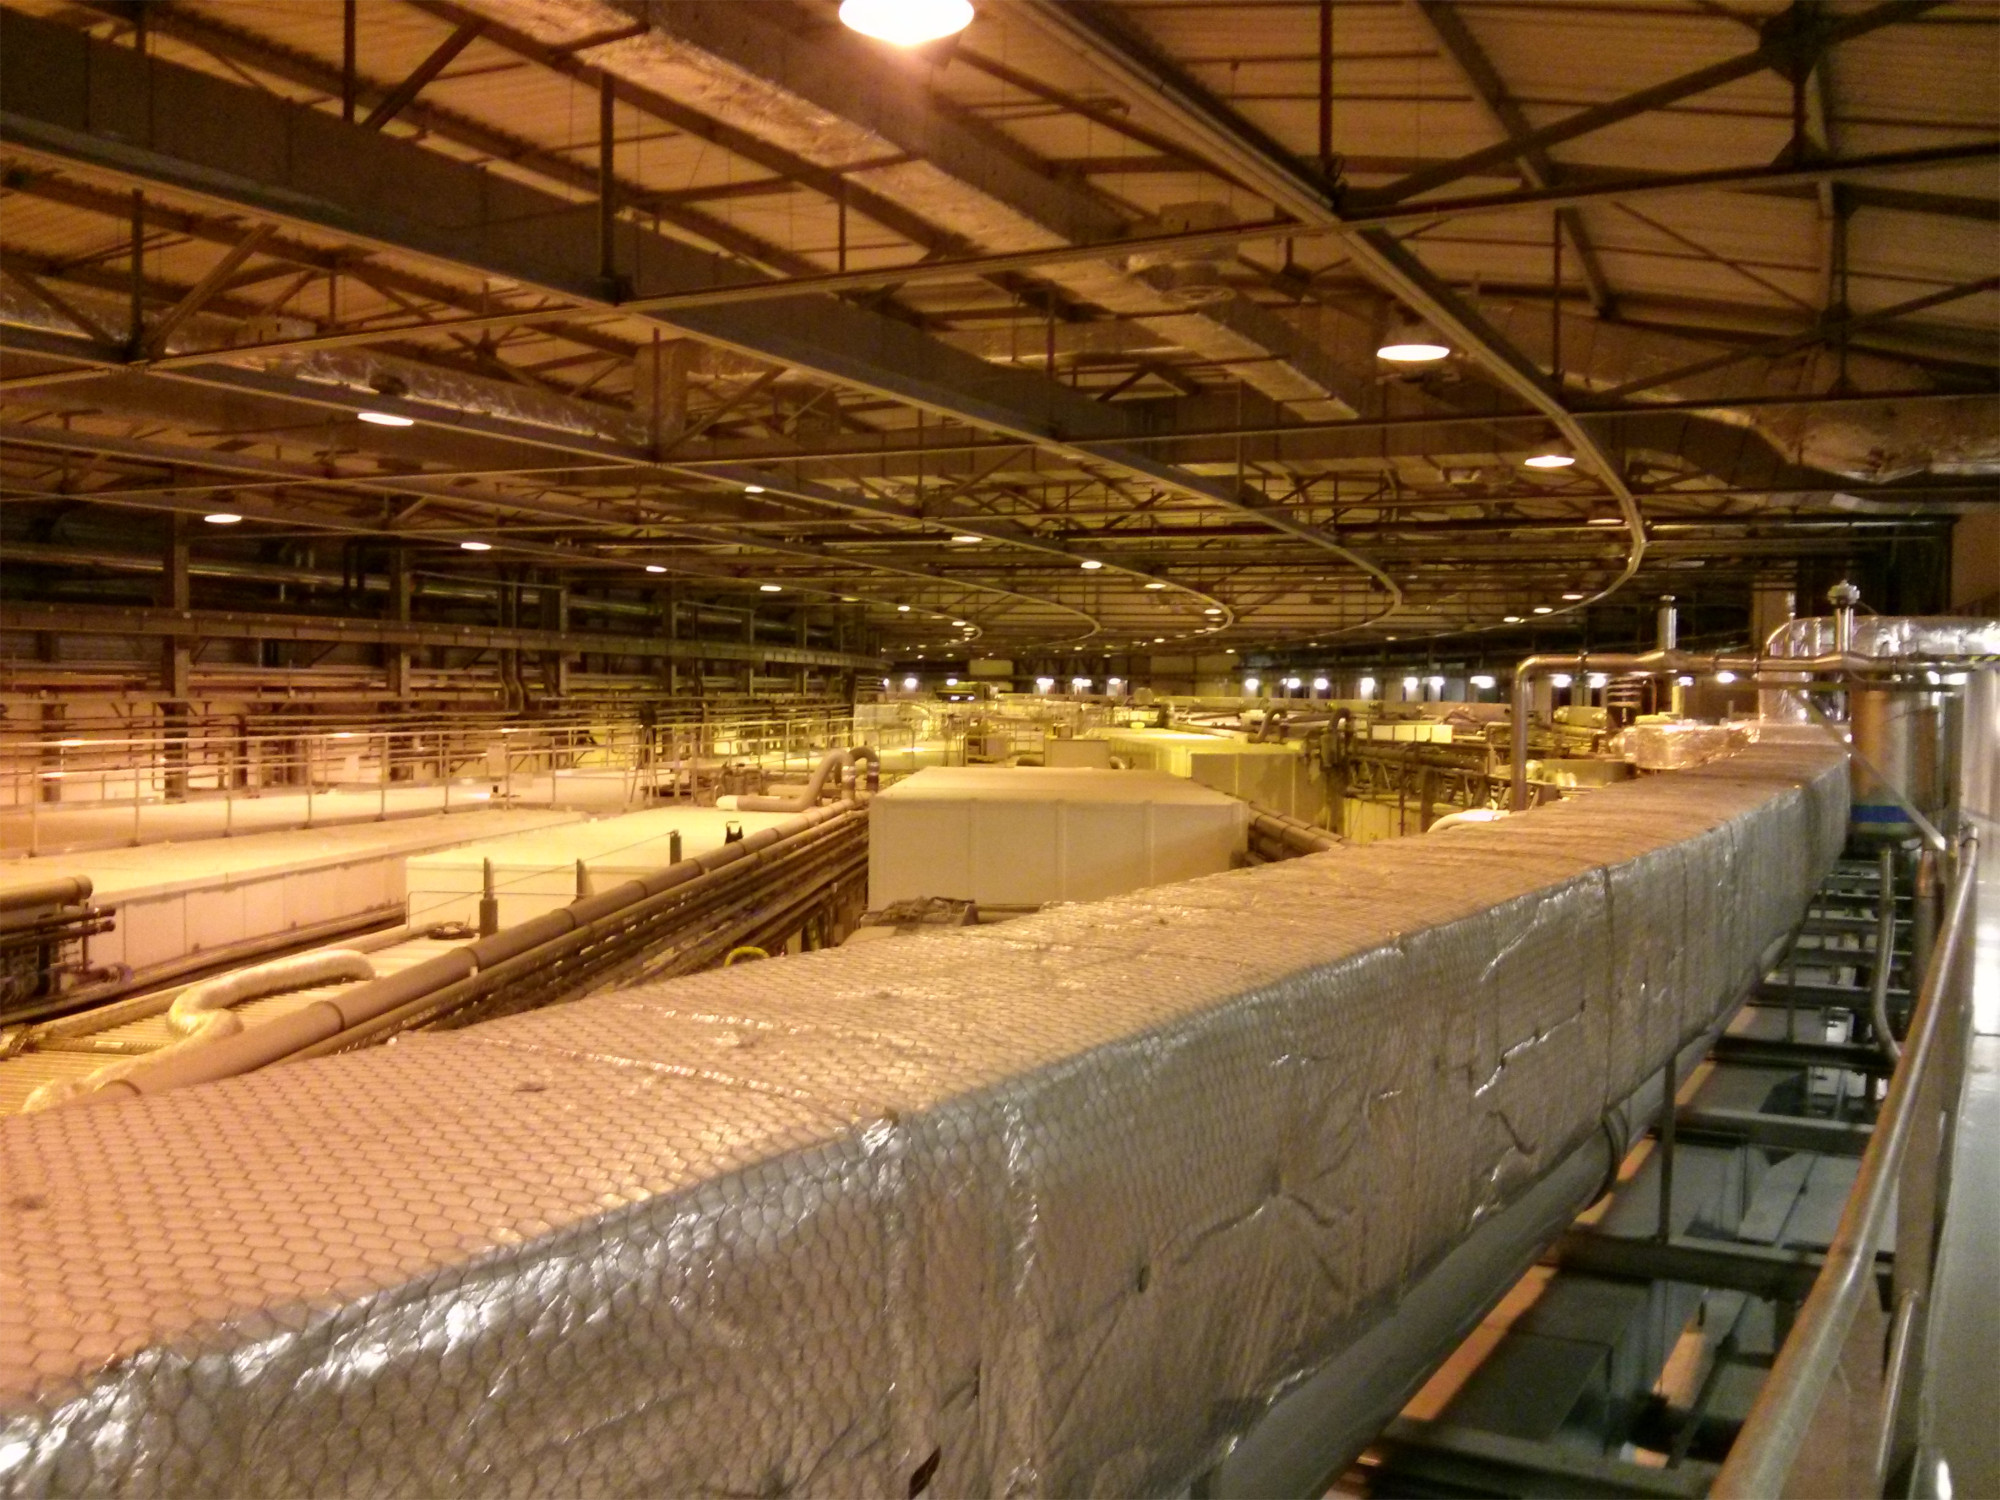
\includegraphics[width=0.8\textwidth]{Images/IMG_20151210_213319.jpg}
        \caption{Hall of experiments (ESRF Grenoble)}
        \label{Hall}
    \end{center}
\end{figure}
\medskip

On the figure \ref{Incident}, you can see the beginning of the beamline used (BM23) the tunnel on the right is the exit of storage ring and the first component focus X-ray beam in the beamline.


\begin{figure}[H]
    \begin{center}
        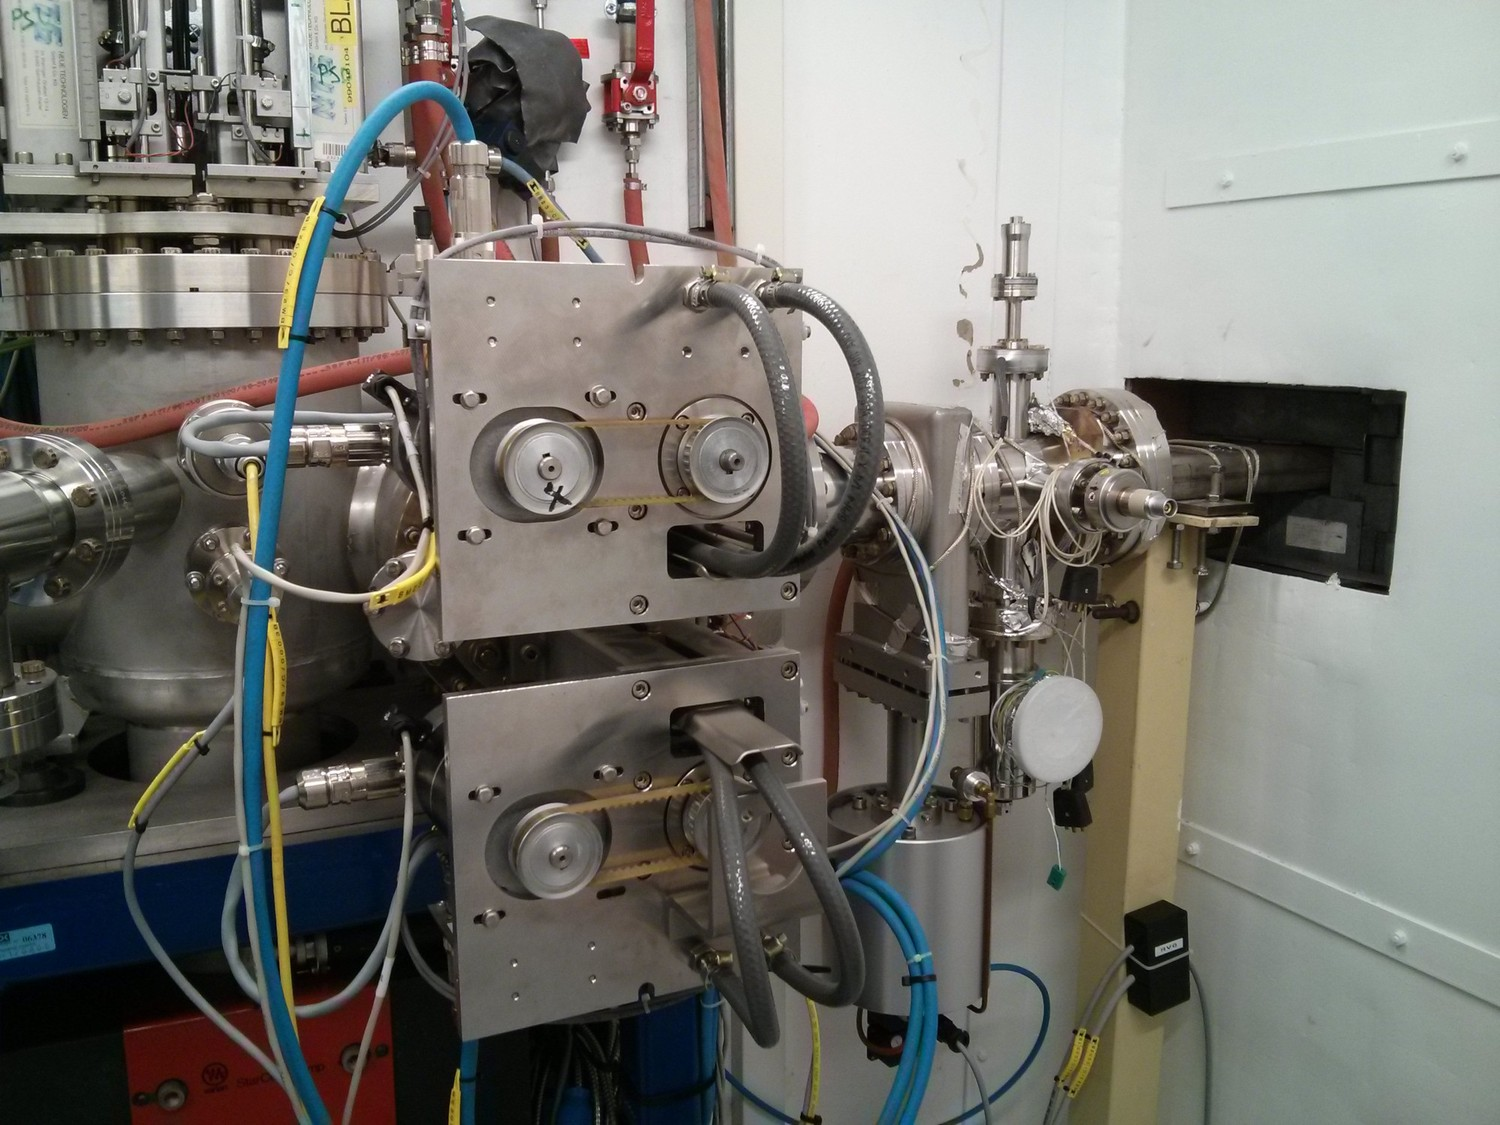
\includegraphics[scale=0.13]{Images/IMG_20151210_202655.jpg}
        \caption{Beamline enter for X-ray radiation and focus beam straight in the beamline}
        \label{Incident}
    \end{center}
\end{figure}
\medskip

The first insteresting component is the monochromator on figure \ref{monochromateur}. When the breaking radiation is created, it got a wide band of energy, the monochromator used Bragg reflection to keep only X-rays of energy selected. Bragg's law is the equation \ref{Bragg}. This equation show that the dispertion in wavelength $\lambda$ cause a dispertion in reflection angle. The monochromator use this to shut down X-rays that don't have the right energy.

\begin{equation}
    2d sin \theta = n \lambda  \label{Bragg}
\end{equation}
Avec:\\
d: distance between the two mirors\\
$\theta$: reflection angle\\
n: diffraction order\\
$\lambda$: wavelength\\
\medskip
\begin{figure}[H]
    \begin{center}
        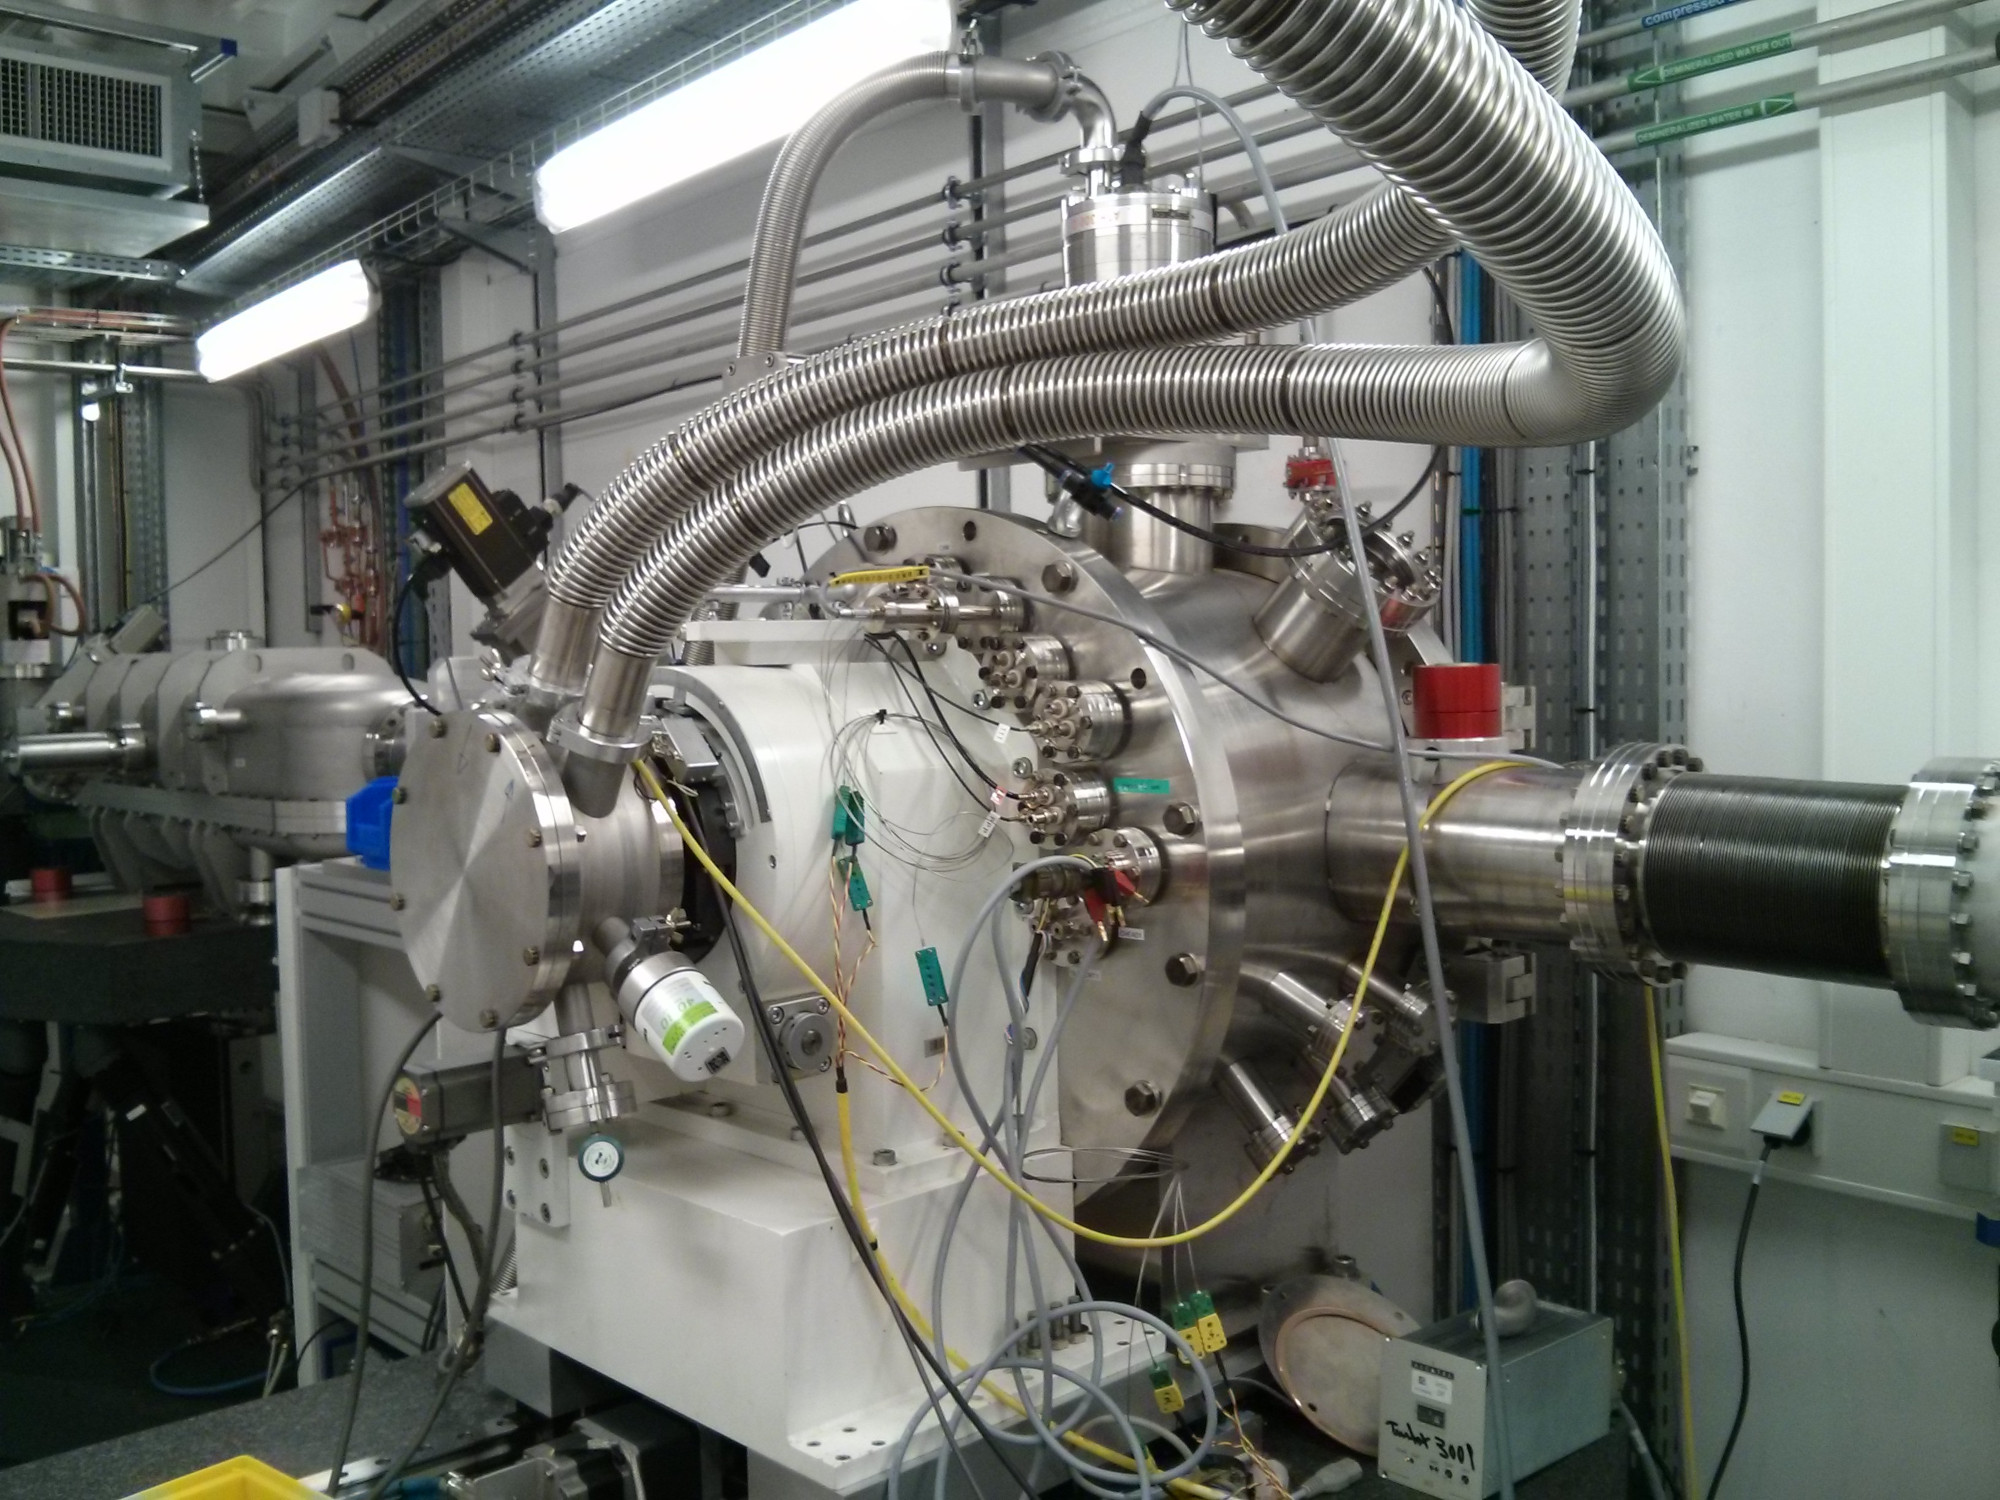
\includegraphics[scale=0.13]{Images/IMG_20151210_202721.jpg}
        \caption{Monochromator}
        \label{monochromateur}
    \end{center}
\end{figure}
\medskip

Just after the monochromator, it is necessary to put a diffraction grating (figure \ref{Reseau_diffract}) to select only the first diffraction order n=1 (delete harmonics).

\begin{figure}[H]
    \begin{center}
        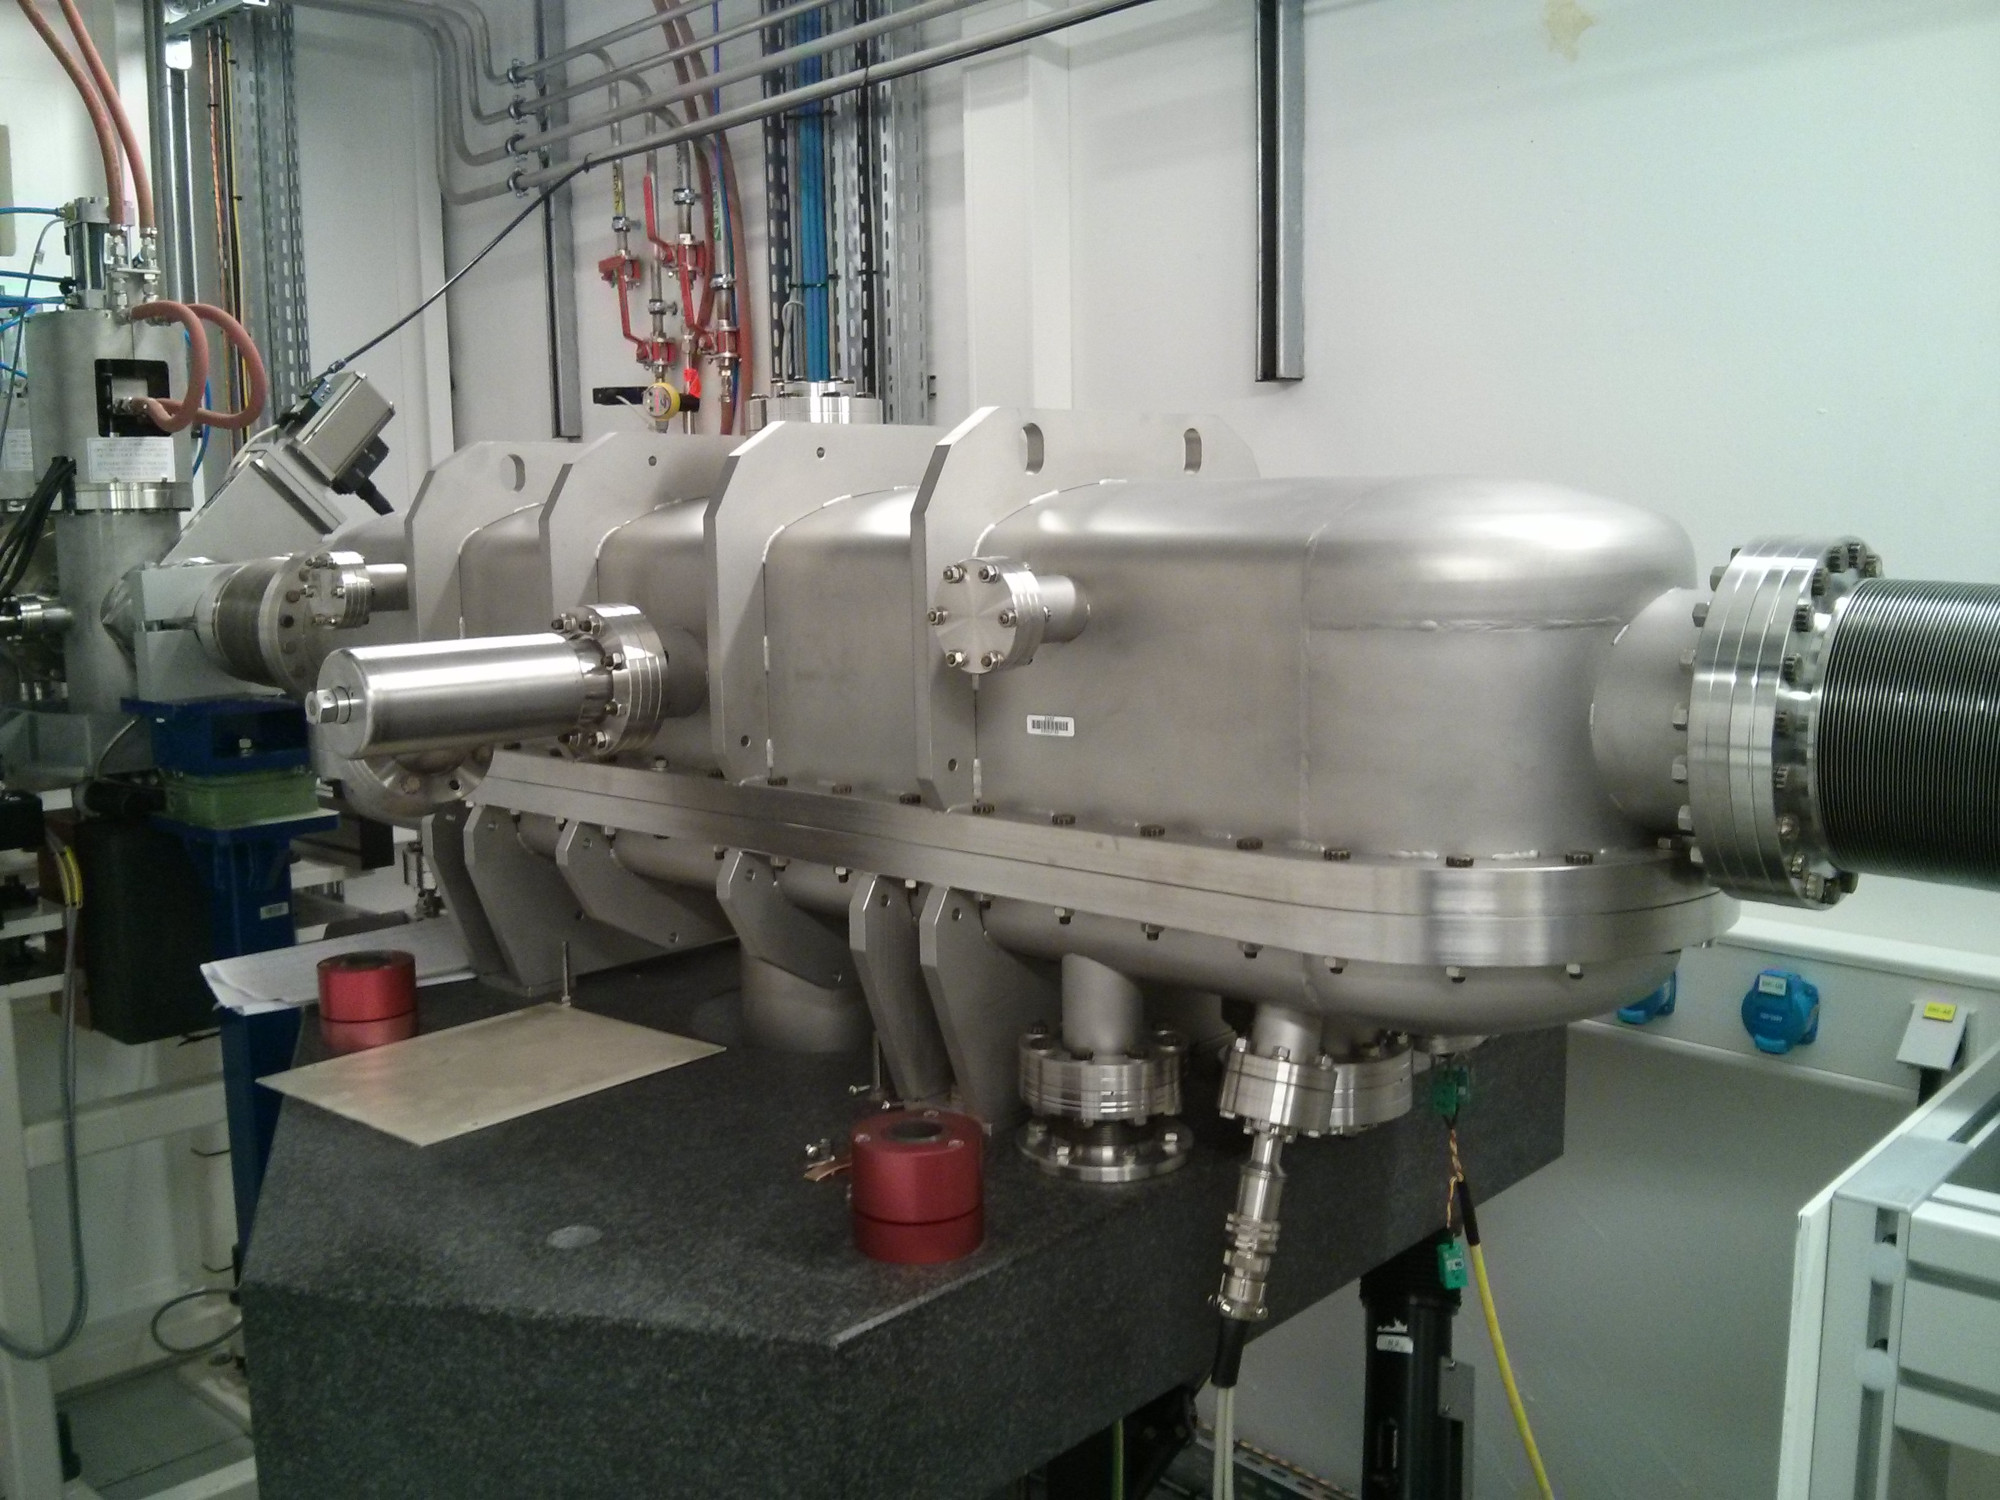
\includegraphics[scale=0.11]{Images/IMG_20151210_202740.jpg}
        \caption{Diffraction grating}
        \label{Reseau_diffract}
    \end{center}
\end{figure}
\medskip

Now we have got the correct X-ray, the mesure is simple, we just need to put our sample in the beamline (figure \ref{ligne_mesure}) and mesure X-ray intensity before and after passing through the sample. The intensity difference give us the absorption induced by the crossing of our sample.

\begin{figure}[H]
    \begin{center}
        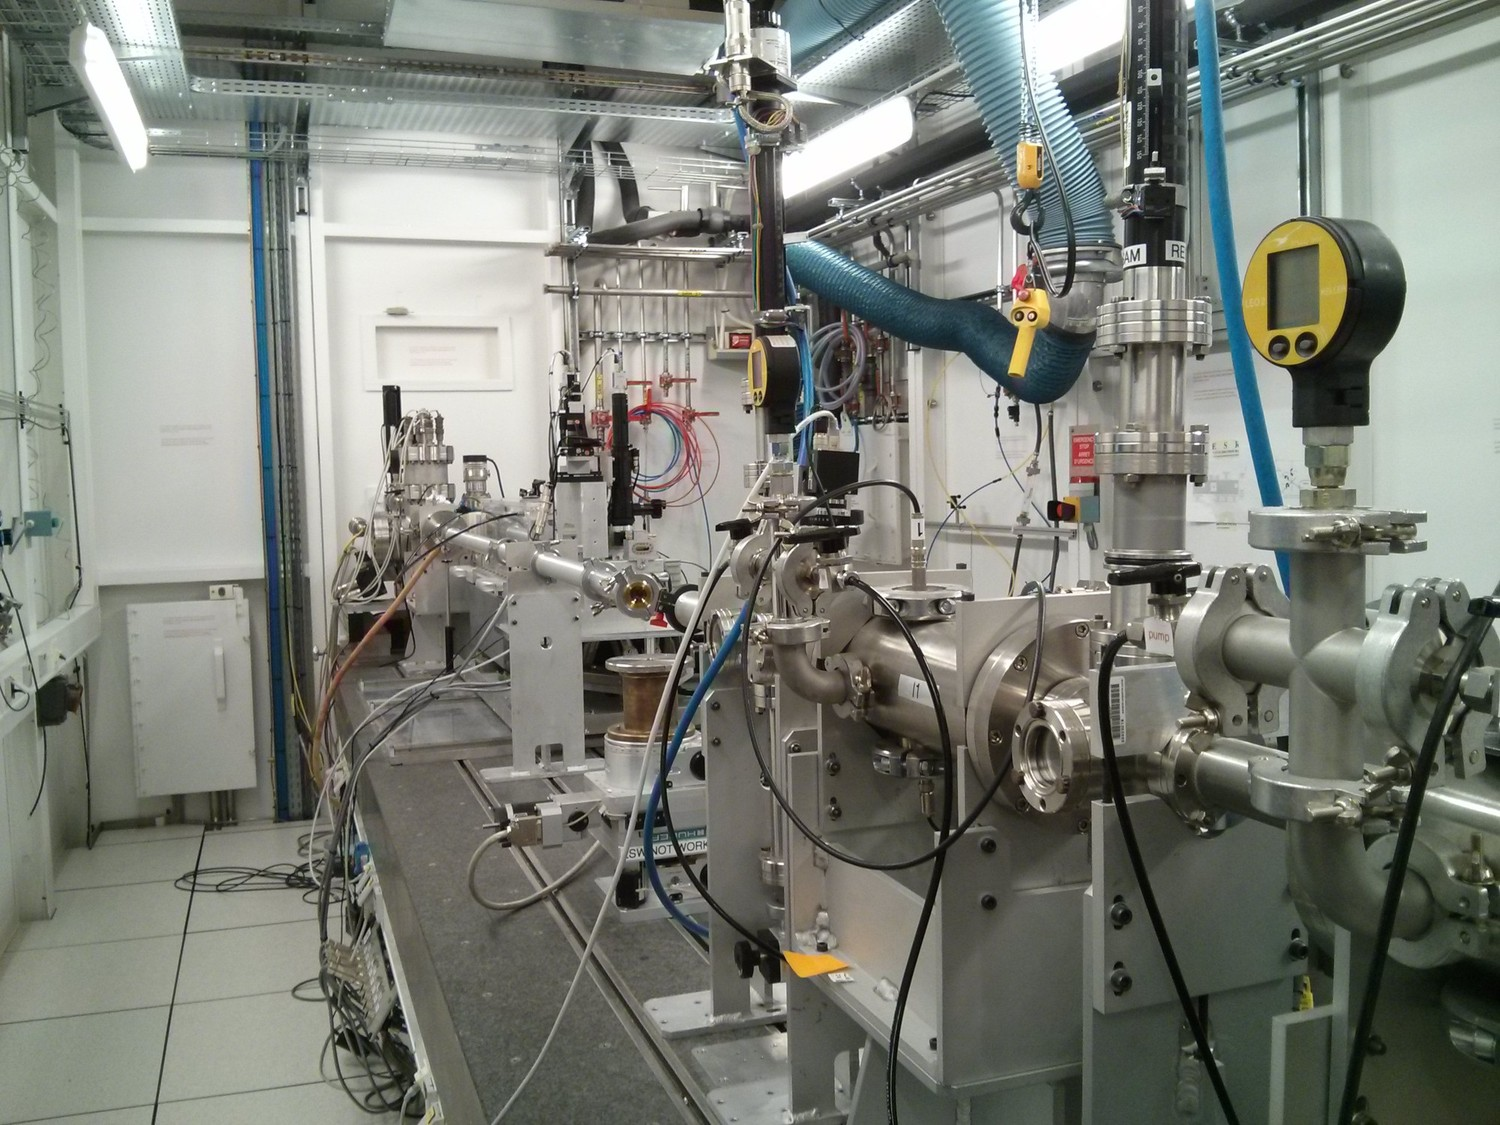
\includegraphics[scale=0.07]{Images/IMG_20151210_203229.jpg}
        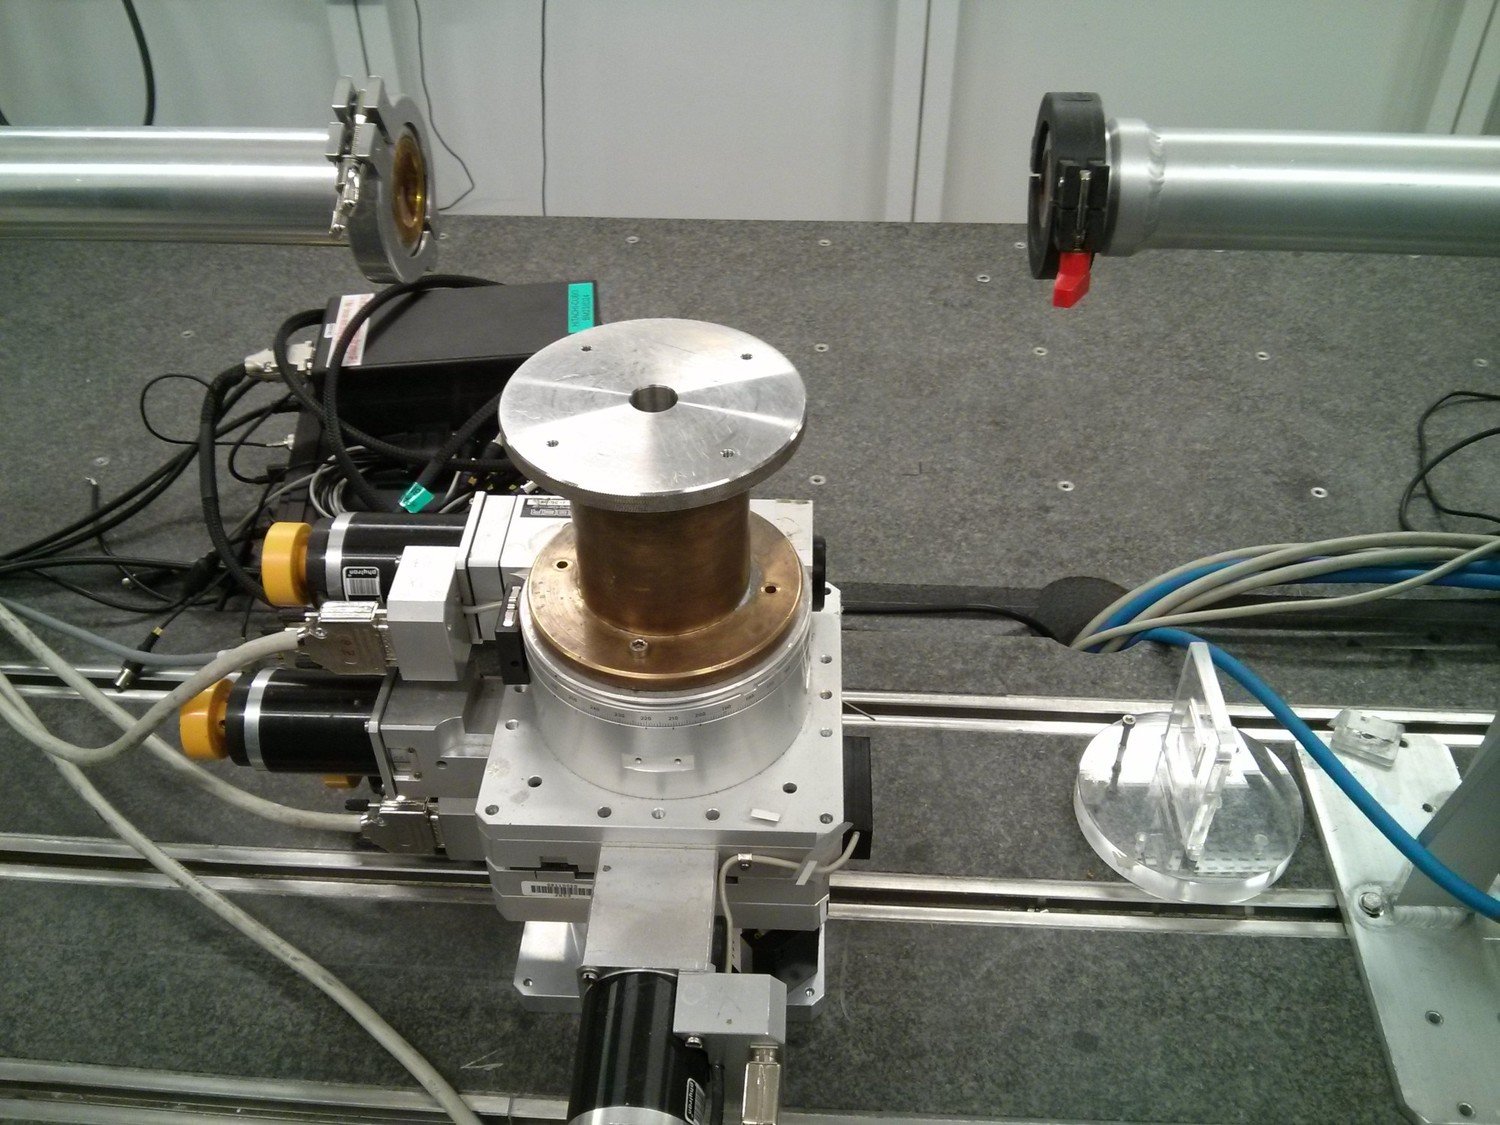
\includegraphics[scale=0.07]{Images/IMG_20151210_203316.jpg}
        \caption{experimental cab}
        \label{ligne_mesure}
    \end{center}
\end{figure}
\medskip


\newpage



\section{Experimental measurements}
\subsection{Reference sample Cu foil}


\subsection{Cu2O sample construction}


\subsection{Graph analysis and results} \label{results}
The different samples presented earlier and another sample of CuO prepared by the first group have all been analysed using the EXAFS technique. The results are presented and discussed below. All these graphs shows the absorption of copper atoms, since oxygen does not absorb X-Ray very well.

\subsubsection{Absorption graph}
The figure \ref{graph1} presents the absorption graph of the three samples. The normalized absorption is plotted versus the X-ray beam energy. Despite they have a similar composition with the same atoms involved, the three samples have a different absorption at the same energy. The influence of neighbouring atoms can be seen in this first plot, and the interaction of the photo-electron generated are quite different depending on the structure of the material.
\begin{figure}[h]
    \begin{center}
        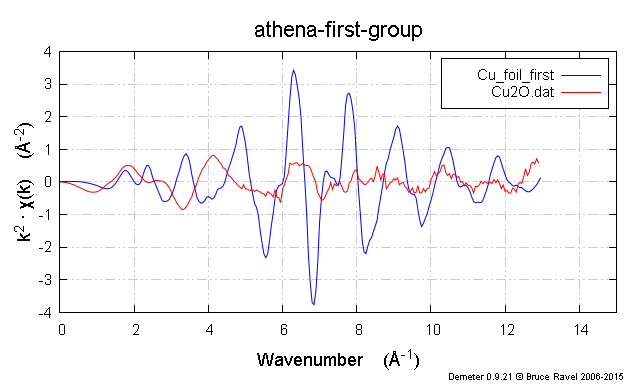
\includegraphics[width=0.7\textwidth]{ImagesTP/image2}
        \caption{}
        \label{graph1}
    \end{center}
\end{figure}

Figure \ref{graph2} shows absorption function plotted versus wavenumber k. The dependence between the energy and the wavenumber of the X-ray is given by   with Wk the ionization energy of the atom.
Absorption also depends strongly on the material analysed. The pure Cu foil (red curve) shows oscillations with a much higher amplitude than the two oxides. The two oxides signals also present an important noise, especially CuO. The explanation can be a non-uniformity of the concentration of CuO in the sample.
\begin{figure}[h]
    \begin{center}
        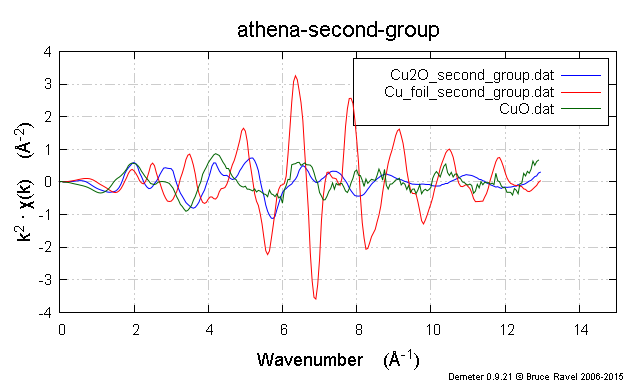
\includegraphics[width=0.7\textwidth]{ImagesTP/image4}
        \caption{}
        \label{graph2}
    \end{center}
\end{figure}

\subsubsection{Neighbours distance graph}
Now the previous curves can be used to check which neighbours does copper atoms see in the structure of the material. A Fourier transform is performed on the absorption function curves (Fig.\ref{graph2}). So the absorption can now be plotted versus a radial distance as shown in figure \ref{graph3}. The curves obtained have all several peak corresponding to the interaction between the photo-electron and the different neighbours of copper atoms in the structure. To find out which peak correspond to which interaction, these curves are crossed with a database which can be found online. Every interaction between copper and other atoms has his own signature previously measured and classified. That means that the interactions must be predicted depending on the analysed sample. These interactions are then checked one by one.



\begin{figure}[h]
    \begin{center}
        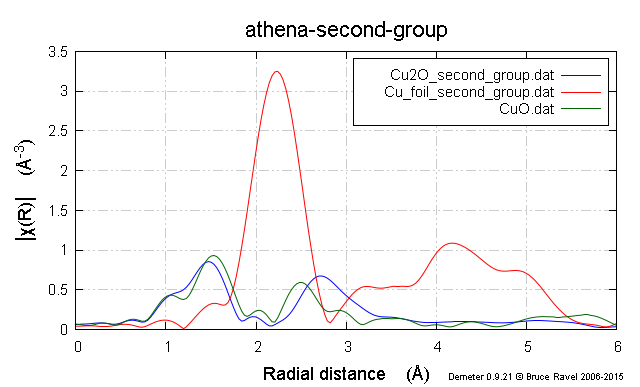
\includegraphics[width=0.7\textwidth]{ImagesTP/image6}
        \caption{}
        \label{graph3}
    \end{center}
\end{figure}


First of all, let’s have a closer look to the copper foil curve. Since the sample only contains copper, it seems obvious to consider the interaction between two copper atoms, where the photo-electron goes to another copper atom then comes back to the first copper atom. The figure \ref{graph4} shows in red this interaction compared to the Cu foil EXAFS curve. There is a match between the Cu foil higher peak and Cu1.1 interaction curve. The peaks on the left of this main peak seems to be explainable with this interaction too. But the right part of the curve does not match really well. However, it can be explained by other interaction between three or more copper atoms, or with the second or more nearest copper atom. The photo-electron can for example go to a second copper atom, then to a third and back to the first. These interactions have been checked and confirmed, but are not plotted in this report.

\begin{figure}[h]
    \begin{center}
        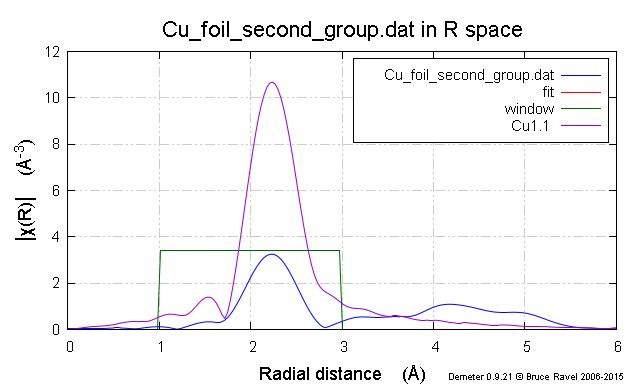
\includegraphics[width=0.7\textwidth]{ImagesTP/image7}
        \caption{}
        \label{graph4}
    \end{center}
\end{figure}

The same analysis has been made with the Cu2O oxide sample, the results are plotted on figure \ref{graph5}. The same interaction between two coppers is checked, along with the interaction between a copper atom and an oxygen atom. As predicted, there is a match for both of them. The two main peaks of the oxide curve, along with the one between them, correspond to the green or purple curve. With the same idea than with the copper foil, the rest of the curve is explained by more complicated interactions, with an atom of copper and then an atom of oxygen for example.
\begin{figure}[h]
    \begin{center}
        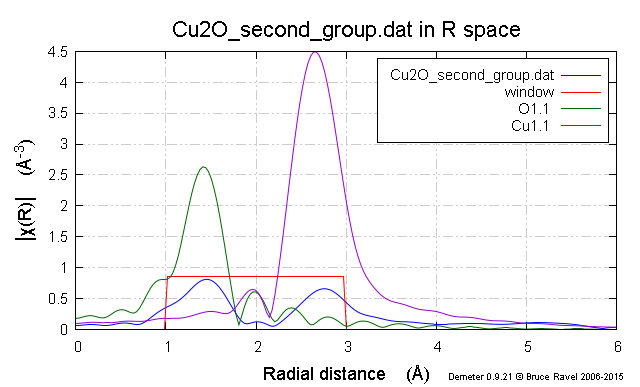
\includegraphics[width=0.7\textwidth]{ImagesTP/image8}
        \caption{}
        \label{graph5}
    \end{center}
\end{figure}



\clearpage
\newpage

\section*{Conclusion}
\addcontentsline{toc}{section}{Conclusion}

	By this study, we have learn a lot about operation of synchrotron and make a real experiment of our matter material caracterization. Moreover, the ESRF it is a great experience in our engineer studies.\smallskip
	
	Result of this study bring out EXAFS phenomenon by caracterization of a Cu$_2$O sample, we have compared spectral absorption of our sample to a Cu sample reference and data files and then recover the composition of our sample.


\nocite{*}
\bibliographystyle{unsrt}
\bibliography{Biblio}
\end{document}
